\section{Results}

To evaluate our methods, we constructed two set of experiments.
In a first set of experiments, we evaluate the separability of the latent representation and the coherence of the generated samples using three labels from the dataset: "Lung Opacity", "Pleural Effusion" and "Support Devices".

\subsection{Evaluation of the latent representation}
%The random performance lies at \py{boilerplate.read_rand_perf()}.\\

%Blurry generated samples is a known problem for VAEs: \cite{zhao2017towards}

\begin{table}
\caption{Generation coherence for MNIST-SVHN-Text. For conditional generation, the letter above the horizontal line indicates the modality which is generated based on the subsets $\sX_k$ below. We report the mean values over 5 runs. Standard deviations are included in  \Cref{subsec:app_mst_results}.}
\label{tab:mst_generation_coherence}
\begin{center}
\begin{small}
    \begin{sc}
    \begin{tabular}{lcccccccccc}
        &  & \multicolumn{3}{c}{M} & \multicolumn{3}{c}{S} & \multicolumn{3}{c}{T} \\
        \cmidrule(l){3-5} \cmidrule(l){6-8} \cmidrule(l){9-11}
        Model & Joint & S & T & S,T & M & T & M,T & M & S & M,S \\
        \midrule
        MVAE & 0.12 & 0.24 & 0.20 & 0.32 & \textbf{0.43} & 0.30 & \textbf{0.75} & 0.28 & 0.17 & 0.29 \\
        MMVAE & 0.28 & \textbf{0.75} & \textbf{0.99} & 0.87 & 0.31 & 0.30 & 0.30 & \textbf{0.96} & \textbf{0.76} & 0.84 \\
        MoPoE & \textbf{0.31} & 0.74 & \textbf{0.99} & \textbf{0.94} & 0.36 & \textbf{0.34} & 0.37 & \textbf{0.96} & \textbf{0.76} & \textbf{0.93} \\
    \end{tabular}
    \end{sc}
\end{small}
\end{center}
\end{table}

%\begin{tabular}{llrrrrrr}
\begin{table}[]
    \centering


\begin{small}
    \begin{sc}
\begin{tabular}{lccccccc}
      &         & \multicolumn{3}{c}{L,F} & \multicolumn{3}{c}{L,F,T} \\
    \cmidrule(l){3-5} \cmidrule(l){6-8}
     MODEL &    LABEL     &         F &         L &         T &         F &         L &         T \\

\midrule
MoPoE & Finding &  0.583445 &  0.542405 &  0.425305 &  0.573645 &  0.530734 &  0.387222 \\

\end{tabular}
    \end{sc}
\end{small}
\end{table}

hi this is another table


\begin{tabular}{llrrrrrrrrr}
\toprule
      &         & \multicolumn{3}{l}{F} & \multicolumn{3}{l}{L,F} & \multicolumn{3}{l}{L,F,T} \\
      &         &      F &      L &      T &     F &      L &      T &      F &     L &      T \\
MODEL & LABEL &        &        &        &       &        &        &        &       &        \\
\midrule
MoPoE & Finding &  0.565 &  0.553 &  0.509 &  0.56 &  0.517 &  0.498 &  0.567 &  0.51 &  0.521 \\
\bottomrule
\end{tabular}

\begin{tabular}{llrrrrrrrrr}
\toprule
      &         & \multicolumn{3}{l}{L} & \multicolumn{3}{l}{L,F} & \multicolumn{3}{l}{L,F,T} \\
      &         &      F &      L &      T &     F &      L &      T &      F &     L &      T \\
MODEL & LABEL &        &        &        &       &        &        &        &       &        \\
\midrule
MoPoE & Finding &  0.514 &  0.518 &  0.536 &  0.56 &  0.517 &  0.498 &  0.567 &  0.51 &  0.521 \\
\bottomrule
\end{tabular}

\begin{tabular}{llrrrrrrrrr}
\toprule
      &         & \multicolumn{3}{l}{T} & \multicolumn{3}{l}{L,F} & \multicolumn{3}{l}{L,F,T} \\
      &         &      F &      L &      T &     F &      L &      T &      F &     L &      T \\
MODEL & LABEL &        &        &        &       &        &        &        &       &        \\
\midrule
MoPoE & Finding &  0.531 &  0.523 &  0.513 &  0.56 &  0.517 &  0.498 &  0.567 &  0.51 &  0.521 \\
\bottomrule
\end{tabular}


\begin{small} \begin{sc}\begin{tabular}{lcccccccccc}

      &         & \multicolumn{3}{c}{F} & \multicolumn{3}{c}{L,F} & \multicolumn{3}{c}{L,F,T} \\  \cmidrule(l){3-5} \cmidrule(l){6-8} \cmidrule(l){9-11} MODEL &    LABEL     &         F &         L &         T &         F &         L &         T &         F &         L &         T \\\midrule
MoPoE & Finding &  0.565 &  0.553 &  0.509 &  0.56 &  0.517 &  0.498 &  0.567 &  0.51 &  0.521 \\

\end{tabular}
\end{sc} \end{small}


Yo, hell othere

Shengjia Zhao et al. \cite{zhao2017towards} show that using a Gaussian prior, the optimal reconstruction is an average of $\approxdistr$ and $\sum _i Var _{\approxdistr} [x_i]$ measures the reconstruction loss.

%\py{
%    pytex_tab(
%    script='scripts/lr_table.py',
%    label='lr_table',
%    caption='Evaluation of the latent representation.',
%    options_pre='\\centering \\resizebox{0.9\\textwidth}{!}{',
%    options_post='}',
%    )
%}
%\vspace{0.4em}
%
%\py{
%    pytex_tab(
%    script='scripts/clf_table.py',
%    label='clf_table',
%    caption='Evaluation of the classifiers.',
%    options_pre='\\centering \\resizebox{0.5\\textwidth}{!}{',
%    options_post='}',
%    )
%}
%\vspace{0.4em}
%
%\begin{figure}
%    \centering
%    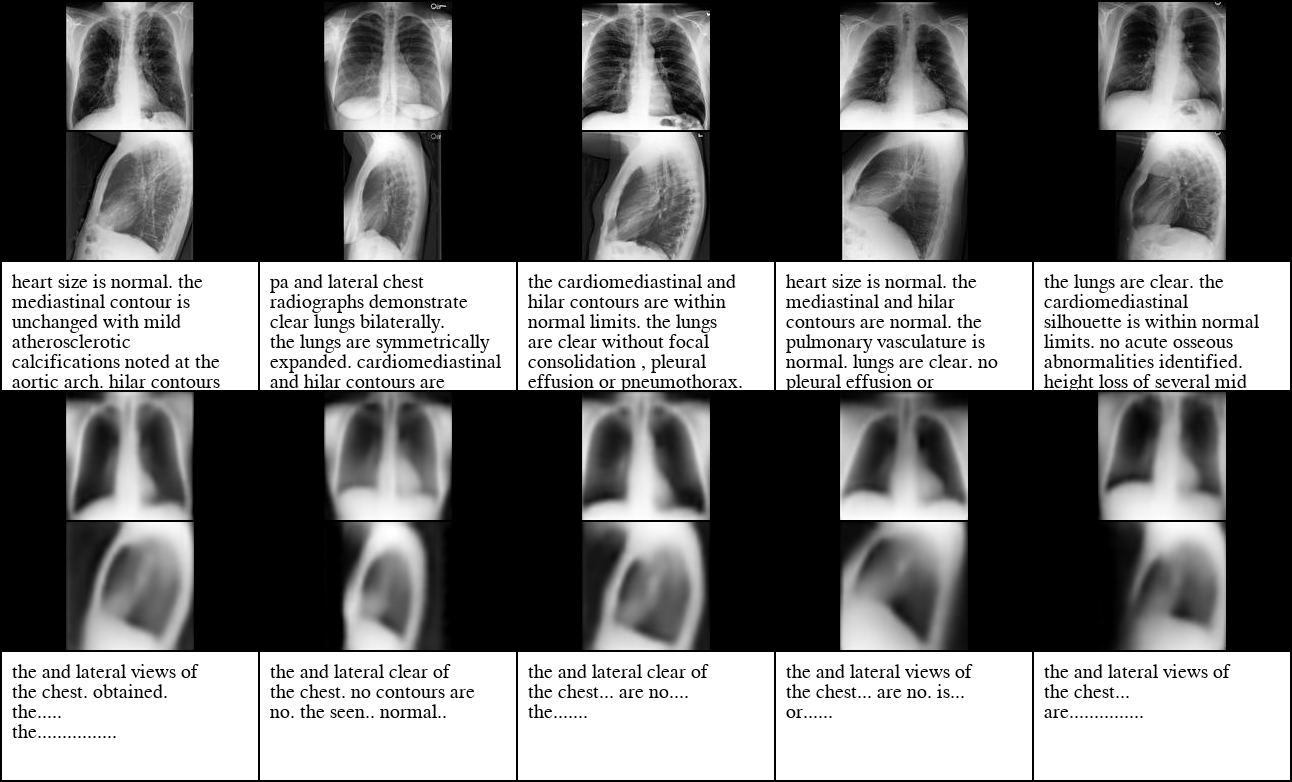
\includegraphics[width=\textwidth]{data/cond_gen/Lateral_PA}
%    \caption{
%        Lateral and PA as conditioner.
%    }
%    \label{fig:fig_cond_latPA}
%\end{figure}
%
%\py{
%    pytex_tab(
%    script='scripts/gen_eval_table.py',
%    label='gen_eval_table',
%    caption='Evaluation of the generation coherence.',
%    options_pre='\\centering \\resizebox{1.1\\textwidth}{!}{',
%    options_post='}',
%    )
%}
%\vspace{0.4em}